% How to use:
% Your computer must know where to look for the cite.sty and graphics.sty libraries,
% as well as the plain.bst style file.  It should probably have these by default, but
% if you are getting errors then it is something to look into.
% In order to compile, run:
% latex templatefortechnicalreports
% bibtex templatefortechnicalreports
% latex templatefortechnicalreports
% latex templatefortechnicalreports
% If you have everything ready, this should produce a dvi which you can convert to ps or pdf.
% If you are having trouble with the alignment of graphics, try first converting dvi->ps then ps->pdf.

\documentclass[12pt]{article}
\usepackage{cite}
\usepackage{graphicx}
 \usepackage{float}
\usepackage[top=1.5in,bottom=1in,right=1in,left=1in]{geometry}
\usepackage{url}
\usepackage{amsmath}

\usepackage{color}
\usepackage{listings}
\lstset{ %
language=matlab,                % choose the language of the code
basicstyle=\footnotesize,       % the size of the fonts that are used for the code
numbers=left,                   % where to put the line-numbers
numberstyle=\footnotesize,      % the size of the fonts that are used for the line-numbers
stepnumber=1,                   % the step between two line-numbers. If it is 1 each line will be numbered
numbersep=5pt,                  % how far the line-numbers are from the code
backgroundcolor=\color{white},  % choose the background color. You must add \usepackage{color}
showspaces=false,               % show spaces adding particular underscores
showstringspaces=false,         % underline spaces within strings
showtabs=false,                 % show tabs within strings adding particular underscores
frame=single,           % adds a frame around the code
tabsize=2,          % sets default tabsize to 2 spaces
captionpos=b,           % sets the caption-position to bottom
breaklines=true,        % sets automatic line breaking
breakatwhitespace=false,    % sets if automatic breaks should only happen at whitespace
escapeinside={\%*}{*}          % if you want to add a comment within your code
}

\begin{document}
%%%%%%%%%%%%%%%%%%%%%%%%%%%%%%%%%%%%%%%%%%%%%%%%%%%%%%%%%%%%%%
%%%%%%%%%%%%%%%%%%%%%%%%%%%%%%%%%%%%%%%%%%%%%%%%%%%%%%%%%%%%%%
%%%%%%%%%%%%%%%%%%%%%%%%%%%%%%%%%%%%%%%%%%%%%%%%%%%%%%%%%%%%%%
\begin{titlepage}
\begin{center}
\LARGE ME759 Final Project\\
\vspace{1.0in}
\Large Diagonally Dominant Banded Systems Solving with CUDA\\
\vspace{2.0in}
\mdseries Elliott Biondo \\
\vfill
December 15, 2013
\end{center}
\end{titlepage}

%%%%%%%%%%%%%%%%%%%%%%%%%%%%%%%%%%%%%%%%%%%%%%%%%%%%%%%%%%%%%%
\newpage
\begin{abstract}

Partial differential equations are often solved numerically, which may involve
a step where it is necessary to solve a system of equations that can be
represented by:

$$
Ax=b
$$

where $A$ is a diagonally dominant banded matrix and $b$ provides multiple
right-hand sides (RHS). In this project, a program was written to solve this
system on an Nvidia GPU using CUDA. The program uses parallel implementations
of LU decomposition, followed by forward and backward substitution. The program
only stores and operates on the band of the matrix. Scaling analysis indicates
that this program is systematically faster than the Intel MKL banded
matrix solver (\texttt{dgbsv}) over a range of matrix dimensions and bandwidths and a
single RHS. However, MKL outperforms the CUDA program when a large number
of RHS are used. Visual profiling using NVVP indicates a potential for further
parallelization of the forward and backward solving steps, which dominant the
execution time.

This report also explores an OpenMP banded solver program, which also only
stores and operates upon the matrix band. It is shown that naively using OpenMP
threads for the same purpose of CUDA threads does not result in
speedup. The only meaningful parallelization achieved with OpenMP involved
parallelizing the solving of multiple RHS. The resulting program is faster than
the CUDA program for multiple RHS, but still slower than MLK.

Keywords: CUDA, linear system, band matrix, MKL, OpenMP
\end{abstract}

%%%%%%%%%%%%%%%%%%%%%%%%%%%%%%%%%%%%%%%%%%%%%%%%%%%%%%%%%%%%%%
\newpage
\tableofcontents
%%%%%%%%%%%%%%%%%%%%%%%%%%%%%%%%%%%%%%%%%%%%%%%%%%%%%%%%%%%%%%
\newpage
\section{Introduction}
\label{sec:introduction}

Science, engineering, and financial applications often give rise to partial
differential equations that are either too difficult or too computationally
expensive to solve analytically. This necessitates the use of numerical
methods in order to obtain an approximate solution. Many such methods involve
discretizing one or more variables in order to obtain a system of linear algebraic
equations in the form:

\begin{equation}
\label{Axb}
Ax=b.
\end{equation}

In Equation \ref{Axb}, $A$ is an $N$ x $N$ matrix and $b$ is  an $N$ x $M$
matrix. The solution is of Equation \ref{Axb} is $x$, an $N$ x $M$ matrix. One
way of solving equation \ref{Axb} is by LU decomposition. $A$ is first
decomposed into a lower triangular matrix ($L$) and an upper triangular matrix
($U$) such that:

\begin{equation}
\label{LU}
A = LU
\end{equation}

The system is then solved in two consecutive steps, first a forward substitution step:
\begin{equation}
\label{forward}
Ly_i = b_i,
\end{equation}

then a backward substitution step:

\begin{equation}
\label{backward}
Ux_i = y_i.
\end{equation}

In Equation \ref{forward}, $b_i$ is the $i^{th}$ column of $b$, which yields
the solution to the intermediate vector $y_i$. In other words, Equations
\ref{forward} and \ref{backward} must be solved to $i$ times to fully solve for
$x$.

It is common for numerical methods to involve a constant $A$ and a
$b$ vector that changes with time (or some other variable). One such example
would be unsteady state diffusion. In these cases, LU decomposition is
advantageous because Equation \ref{LU} can be solved once, and then each
time step will involve the less expensive solving of Equations \ref{forward} and
\ref{backward}. It is also common for $A$ to be a banded matrix of bandwidth $k$. For the
purpose of this report, $k$ is assumed to be equal to

\begin{equation}
\label{half_k}
k = 2 \cdot k_{1/2} + 1,
\end{equation}

where $k_{1/2}$ represents the upper/lower bandwidth, which are presumed
to be equal. Banded matricies may arise if the operator that is being
approximated by $A$ contains some derivative term which is treated with some
finite difference stencil. These systems are often strictly diagonally
dominant, in other words:

\begin{equation}
|a_{ii}| > \sum\limits_{i \neq j} |a_{ij}| \hspace{0.5cm} \mbox{for all i}
\end{equation}


This project implements a parallel solution to Equation \ref{Axb}, presuming $A$
is a diagonally dominant banded matrix and $b$ has multiple right-hand sides (RHS).
This is done using the aforementioned method, on an Nvidia graphics card using
CUDA and also with OpenMP.


%%%%%%%%%%%%%%%%%%%%%%%%%%%%%%%%%%%%%%%%%%%%%%%%%%%%%%%%%%%%%%
\section{Algorithms}
\label{sec:algorithms}

To tackle this problem, a set of mathematical algorithms was first chosen
based on its potential to be parallelized \cite{Heath}. For the chosen set of
algorithms, the matrix is assumed to be strictly diagonally dominate. This
eliminates the need for any pivoting operations. The pseudocode for the LU
decomposition step is seen in Figure \ref{LUcode}. This algorithm modifies the $A$
matrix in place, such that the resulting $L$ and $U$ matrices are embedded
within the original $A$. This avoids the burden of storing the zeros of the
upper portion of $L$ and lower portion of $U$.

\begin{figure}[H]
\caption{Pseudocode for serial LU decomposition. Indexing is done from 0.}
\label{LUcode}
\begin{lstlisting}
  for i = 0 .. n-2
    for j = i+1 .. n-1
      A[j][i] = A[j][i]/A[i][i]
    end
    for j = i+1 .. n-1
      for k = i+1 .. n-1
        A[j][k] = A[j][k] - A[j][i]*A[i][k]
      end
    end
  end
\end{lstlisting}
\end{figure}

The forward solve for $y$ continues as shown in Figure \ref{forwardcode}. The
backward solve for $x$ proceeds as shown in Figure \ref{backwardcode}. It
should be noted that both of these algorithms operate on the A matrix which is
actually the superposition of the L and U, as created by the code in Figure \ref{LUcode}.
These algorithms solve the system in-place, meaning the the final answer for $x$ is stored in $b$.

\begin{figure}[H]
\caption{Pseudocode for the serial forward solve of Equation \ref{forward}.}
\label{forwardcode}
\begin{lstlisting}
  for i = 0 .. n-1
    for j = i+1 .. n-1
      b[j] = b[j] - b[i]*A[j][i]
    end
  end
\end{lstlisting}
\end{figure}

\begin{figure}[H]
\caption{Pseudocode for the serial backward solve of Equation \ref{backward}.}
\label{backwardcode}
\begin{lstlisting}
  for i = n-1 .. 0
    b[i] = b[i]/A[i][i]
    for j = 0 .. i-1
      b[j] = b[j] - b[i]*A[j][i]
    end
  end
\end{lstlisting}
\end{figure}

%%%%%%%%%%%%%%%%%%%%%%%%%%%%%%%%%%%%%%%%%%%%%%%%%%%%%%%%%%%%%%
\subsection{Band Storage}
\label{band}

The algorithm described in Figure \ref{LUcode} preserves the band of $A$ in
creation of the $L$ and $U$ matrices. This allows this algorithm to utilize
band storage. Using band storage, the algorithm must be implemented in a way
such that operations are only done on the band. This complicates the indexing
of the algorithms in Figures \ref{LUcode}, \ref{forwardcode},
\ref{backwardcode}.  By using band storage the number of stored entries is
reduced from $N \cdot N$ to $N \cdot k$, As shown Figure \ref{bandstorage}.

\begin{figure}[H]
\caption{Normal matrix storage vs. band storage.}
\label{bandstorage}
$$
\left(
\begin{array}{c c c c c c c}
a_{00} & a_{01} & a_{02} & 0 & 0 & 0 & 0\\
a_{10} & a_{11} & a_{12} & a_{13} & 0 & 0 & 0\\
a_{20} & a_{21} & a_{22} & a_{23} & a_{24} & 0 & 0\\
     0 & a_{31} & a_{32} & a_{33} & a_{34} & a_{35} & 0\\
     0 &      0 & a_{42} & a_{43} & a_{44} & a_{45} & a_{46}\\
     0 &      0 &      0 & a_{53} & a_{54} & a_{55} & a_{56}\\
     0 &      0 &      0 &      0 & a_{64} & a_{65} & a_{66}\\
\end{array}
\right)
\rightarrow
\left(
\begin{array}{c c c c c}
     0 &      0 & a_{00} & a_{01} & a_{02}\\
     0 & a_{10} & a_{11} & a_{12} & a_{13}\\
a_{20} & a_{21} & a_{22} & a_{23} & a_{24}\\
a_{31} & a_{32} & a_{33} & a_{34} & a_{35}\\
a_{42} & a_{43} & a_{44} & a_{45} & a_{46}\\
a_{53} & a_{54} & a_{55} & a_{56} & 0     \\
a_{64} & a_{65} & a_{66} & 0      & 0
\end{array}
\right)
$$
\end{figure}

%%%%%%%%%%%%%%%%%%%%%%%%%%%%%%%%%%%%%%%%%%%%%%%%%%%%%%%%%%%%%%
\section{CUDA Implementation}
\label{sec:implimentation}

\subsection{Computational Methods}

The CUDA implementation utilizes the algorithm described in Figures
\ref{LUcode}, \ref{forwardcode}, \ref{backwardcode}, but only operating on the
band of the matrix, which is stored in the band form described in Section
\ref{band}. This presents numerous challenges to being parallelized with CUDA.
For the LU decomposition step show in Figure \ref{LUcode}, iterative kernel
calls were used for the outermost \texttt{for} loop. This was done in order to
impose synchronization between iterations, which is necessary for this
algorithm. This cannot be done using blocks because there is no notion of block
synchronization in CUDA.

For each of these outer iterations, a $k_{1/2}$ by $k_{1/2}$ square chunk of
the matrix is operated on as seen in Figure \ref{active}.

\begin{figure}[H]
\caption{Progression of active chunk (red to blue).}
\label{active}
\centerline{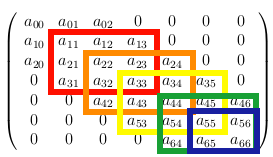
\includegraphics{active_region_colored.png}}
\end{figure}

A 2D tiling strategy was used to perform these operations. This means that the
largest number of operations that can be performed in parallel is $k_{1/2}^2$
which may be poor for small bands. For each outer iteration, 2 sequential steps
must be performed:

\begin{enumerate}
\item{Divide the first number in each row of the active chunk by upper-left-most element.}
\item{Recompute every other value in the active chunk (which depends on step 1).}
\end{enumerate}

Again, since there is no block synchronization in CUDA, two separate kernel
calls were needed for steps 1 and 2. The step 1 kernel involves $k_{1/2}$
active threads. One thread in each block first retrieves the upper-left-most
diagonal element from global memory and stores it in shared memory for the
benefit of the block. Synchronization is performed and then every active thread
must retrieve values from global memory from a different row in the matrix,
which is not coalesced due to row-major storage. The step 2 kernel operates on
the full $k_{1/2}$ by $k_{1/2}$ chunk. Memory access is coalesced (due to band
storage) and no synchronization is required.

For each RHS the forward and backwards substitution steps must also
be performed sequentially, which is done with two similar kernels.  Each is
called $N$ times iteratively for each RHS. Upon each iteration, one
thread per kernel call computes a final value and stores a multiplication
factor in shared memory.  Synchronization is done, then $k_{1/2}$ operations are
performed in parallel, though memory access is not coalesced. Asynchronous
memory copying is used for each RHS. All memory copy operations between
device and host for the entire program utilize pinned host memory.

\subsection{Usage}
\label{usage}

Full build and usage instructions are found in
the file README\_BUILD\_AND\_USAGE. The executable created is called
\texttt{cuda\_solve} and has two modes: one for testing and one for production
runs. For testing, 3 arguments are supplied:

\begin{verbatim}
>> ./cuda_solve <matrix dimension> <bandwidth> <number of RHS> \end{verbatim}

This generates a random diagonally dominant matrix with the supplied dimension
and bandwidth, and also the corresponding RHS (such that all values of $x$ are
unity), and solves the system of equations. The correctness of the solution is
accessed and reported to \texttt{stdout}. Inclusive execution time is output. For production runs, 4
arguments are supplied:

\begin{verbatim}
>> ./cuda_solve <file name A> <file name b> <matrix dimension> <number of RHS>
\end{verbatim}

The file containing matrix A must specify the values of $A$ in row major order
using band storage, whereas the file containing $b$ must be in column major
order. Timing results and the solution ($x$) are printed to \texttt{stdout}.


%%%%%%%%%%%%%%%%%%%%%%%%%%%%%%%%%%%%%%%%%%%%%%%%%%%%%%%%%%%%%%
\section{CUDA Numerical Experiments}
\label{sec:numericalexperiments}

\subsection{Scaling analysis and comparison with INTEL MKL}

All scaling analysis was done on the Euler cluster with a Nvidia GeForce GTX 480 GPU.

\subsubsection{Intel MKL solver}

A program was created using Intel MKL with identical functionality to the test
mode of \texttt{cuda\_solve} as described in Section \ref{usage}. Full build
instructions for the executable \texttt{mkl\_solve} are found in the file
README\_BUILD\_AND\_USAGE. This script utilizes the MKL banded matrix solving kernel,
\texttt{LAPACKE\_dgbsv}.

\subsubsection{Matrix dimension and bandwidth scaling comparison}

Figure \ref{scaling} shows how execution time scales as a function of matrix
dimension ($N$) and bandwidth for a single RHS. The different bandwidths were
used as a percentage of matrix dimension. This figure shows that the CUDA
program is systematically faster than MLK over these dimensions and bandwidths.
The plot suggests that MKL has a higher startup cost than CUDA, which has a
diminishing affect on execution time for high matrix dimensions. The plot also
shows that the discrepancy between CUDA and MKL is largest for small
bandwidths, which is strange since the parallelization of the CUDA algorithm
goes like $k_{1/2}$, as discussed in Section \ref{sec:implimentation}.

\begin{figure}[H]
\caption{CUDA and MKL performance as a function of matrix dimension for different bandwidth percentages and a single RHS. Bandwidth percentages are approximate because bandwidths are odd (as defined by Equation \ref{half_k}). For example, for the N=100 cases, bandwidth of 11 was used for the 10\% cases.}
\label{scaling}
\centerline{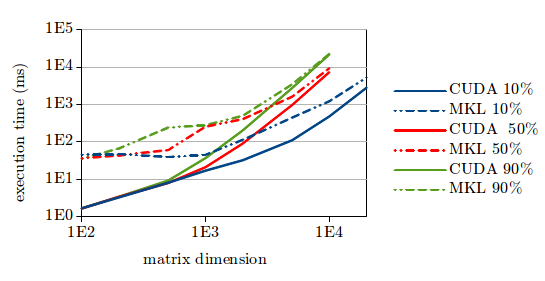
\includegraphics[width=12cm]{full_scaling.png}}
\end{figure}

\subsubsection{Number of right-hand sides scaling comparison}
\label{sec:rhs}

Scaling behavior was also accessed as a function of number of RHS, as seen in
Figure \ref{rhs}. As discussed in Section \ref{sec:implimentation}, the
solving of different RHS is serialized within the CUDA program.
Likewise, the execution time scales linearly with number of RHS. This seems to
also be true for the MKL program for high RHS. However, the slope of the MKL
line is shallower which means that although both programs serialize the forward
and backward substitution, MKL does a better job.

\begin{figure}[H]
\caption{Right hand size scaling analysis. The matrix dimension was kept constant at 1000 with a bandwidth of 501.}
\label{rhs}
\centerline{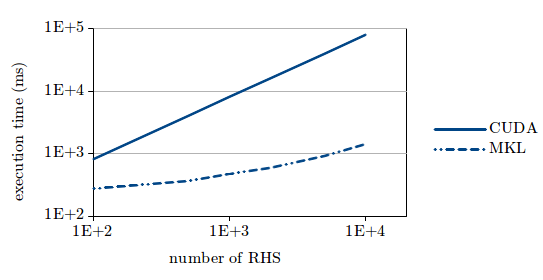
\includegraphics[width=12cm]{rhs.png}}
\end{figure}


\subsection{Profiling with NVVP}

NVVP was run with a matrix dimension 1000, a bandwidth of 501, and 10 RHS.
 Results are shown in Figure \ref{nvvp}. This shows that even with a
modest number of RHS, the forward and reverse substitutions
dominant the execution time. Since the solving of each column in the $b$ matrix is
independent, the implementation could exploit further
parallelization. This would result in a speedup of approximately 2.

\begin{figure}[H]
\caption{NVVP output.}
\label{nvvp}
\centerline{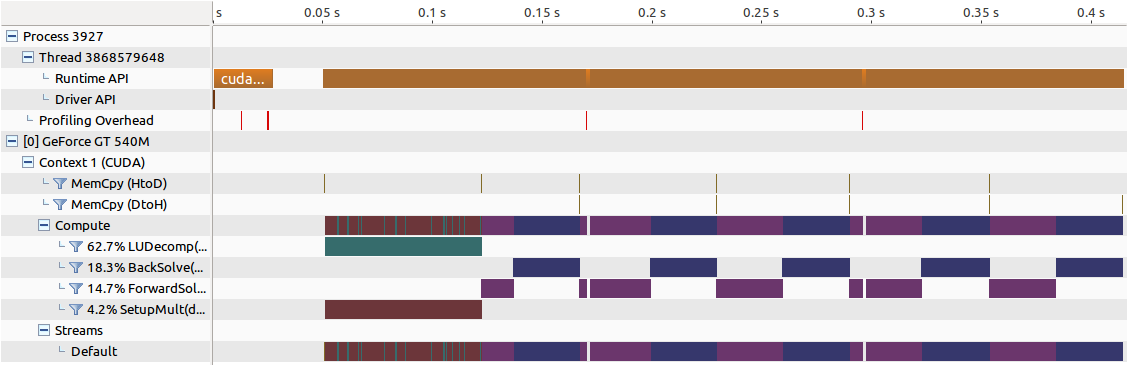
\includegraphics[width=12cm]{nvvp.png}}
\end{figure}

\subsection{CUDA memcheck}

CUDA memcheck was run using a matrix dimension of 1000, a
bandwidth of 501 and 10 RHS. Full output appears in Appendix A. The
memcheck raises two incidences of "Program hit error 17 on CUDA API call to
cudaFree." It is not clear where this error is coming from. This may
indicate that an array is being over-stepped, but this is somewhat unlikely
because the program gives correct results over a large range of dimensions and
bandwidths without segmentation faults. One might suspect that this is arising from the use of pinned host
memory, since two blocks of pinned host memory are used (for arrays $A$ and
$b$).

%%%%%%%%%%%%%%%%%%%%%%%%%%%%%%%%%%%%%%%%%%%%%%%%%%%%%%%%%%%%%%
\section{OpenMP}
\label{sec:omp}

An attempt was also made to implement a banded system solver using OpenMP. This
was done by first creating a serial solver using the algorithms described by
Figures \ref{LUcode}, \ref{forwardcode}, \ref{backwardcode}, on a matrix
stored in banded format.

As it turns out, these algorithms do not offer much opportunity for
parallelization using OpenMP. OpenMP threads have a considerably higher
overhead associated with creation. This makes the tiling  strategy used in CUDA
programming difficult to replicate.  For example, in the CUDA program, LU
decomposition was done by employing blocks to fill an active region of the
matrix. This same strategy was attempted with OpenMP by creating a parallel
\texttt{for} loop (line 5 of Figure \ref{LUcode}) with private index varibles.
This was done (in file \texttt{omp\_solve\_slow.c}), resulting in program that
is considerably slower than the similar serial program.  This is shown in
Figure \ref{slow}.  The problem is, these inner \texttt{for} loops are executed $N-2$
times by the outer for loop, each time with an expensive thread creation step.
Since the axes of Figure \ref{slow} are the same as Figure \ref{scaling} it is easy to
verify that the CUDA and MKL programs are much faster than the serial program.

\begin{figure}[H]
\caption{Scaling analysis for serial and slow OpenMP implementation for 50\% bandwidth. Axes are the same as Figure \ref{scaling}.}
\label{slow}
\centerline{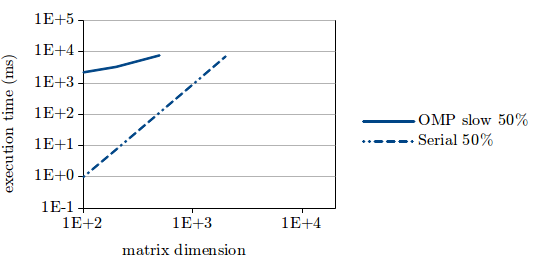
\includegraphics[width=12cm]{slow.png}}
\end{figure}

The same problems associated with paralleling LU decomposition exist when
parallelizing the forward/backward substitution. For this reason, it appears
the only worthwhile way of parallelizing the serial algorithm is by
parallelizing the forward/backward solve of multiple RHS. This was done in file
\texttt{omp\_solve.c}. The matrix dimension and bandwidth scaling for this
program should be identical to the serial program. The RHS scaling is shown in
Figure \ref{omprhs}. This Figure shows that OpenMP offers an order of magnitude
speedup over the serial program. The axes of Figure \ref{omprhs} are the same
as \ref{rhs}. Comparing these figures revels that the OpenMP program is also
considerable faster than the CUDA program, but still slower than the MKL program. In other words, the serial MKL program seems to scale better than even a fully parallel OpenMP implementation.

\begin{figure}[H]
\caption{RHS scaling analysis for OpenMP and serial programs. The matrix dimension was kept constant 1000 with a bandwidth of 501. For OpenMP, the maximum number of threads was used: 16.}
\label{omprhs}
\centerline{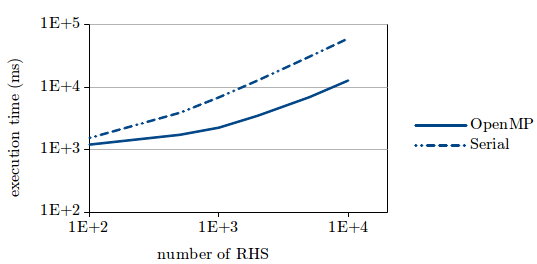
\includegraphics[width=12cm]{omp_rhs.png}}
\end{figure}

%%%%%%%%%%%%%%%%%%%%%%%%%%%%%%%%%%%%%%%%%%%%%%%%%%%%%%%%%%%%%%
\section{Conclusion}
\label{sec:conclusion}

In this project, a CUDA program was created to solve a diagonally dominate
banded system using an algorithm to operate on an $A$ matrix stored in banded
matrix form. The program is systematically faster than the Intel MKL banded
matrix solver for a single RHS, but scales much less favorably for multiple
RHS. NVVP results highlight the potential for improved parallelization of
solving multiple RHS. The algorithm chosen for the CUDA implimentation
does not carry over well into the OpenMP world due to a higher overhead
associated with OpenMP thread creation. For this reason, the only meaningful
parallelization achieved was parallelizing the solving of multiple RHS. Though
this method is proved faster than CUDA, the MKL program is still faster. In order
to achieve better results with OpenMP, exploring entirely different algorithms
may be necessary.

%%%%%%%%%%%%%%%%%%%%%%%%%%%%%%%%%%%%%%%%%%%%%%%%%%%%%%%%%%%%%%
\bibliographystyle{plain}
\bibliography{report}

%%%%%%%%%%%%%%%%%%%%%%%%%%%%%%%%%%%%%%%%%%%%%%%%%%%%%%%%%%%%%%
\newpage
\section{Appendix A: CUDA full memcheck results}

\begin{verbatim}
>> cuda-memcheck ./cuda_solve 11 3 1
Test PASSED
========= CUDA-MEMCHECK
========= Program hit error 17 on CUDA API call to cudaFree
=========     Saved host backtrace up to driver entry point at error
=========     Host Frame:/usr/lib64/nvidia/libcuda.so [0x30af90]
=========     Host Frame:./cuda_solve [0x44036]
=========     Host Frame:./cuda_solve [0x3a02]
=========     Host Frame:/lib64/libc.so.6 (__libc_start_main + 0xfd) [0x1ed1d]
=========     Host Frame:./cuda_solve [0x2dd9]
=========
========= Program hit error 17 on CUDA API call to cudaFree
=========     Saved host backtrace up to driver entry point at error
=========     Host Frame:/usr/lib64/nvidia/libcuda.so [0x30af90]
=========     Host Frame:./cuda_solve [0x44036]
=========     Host Frame:./cuda_solve [0x3a0c]
=========     Host Frame:/lib64/libc.so.6 (__libc_start_main + 0xfd) [0x1ed1d]
=========     Host Frame:./cuda_solve [0x2dd9]
=========
========= ERROR SUMMARY: 2 errors
\end{verbatim}

\end{document}


